\documentclass[manuscript,screen=true]{acmart}
 
 \usepackage[utf8]{inputenc}
 \usepackage{xspace}
 \usepackage{balance}
 \usepackage{amsmath,amsfonts,mathtools,amsthm}
 \usepackage{algorithmic}
 \usepackage{algorithm}
 
 \usepackage{balance}
 \usepackage{amsthm,amsmath,array,colortbl,graphicx,multirow}
 \usepackage{comment}
 \usepackage{balance}
 \usepackage{tikz}
 \usepackage{amsmath}
 \usetikzlibrary{decorations.pathreplacing} %
 \usepackage{algorithm}
 \usepackage[font={footnotesize}]{subcaption}
 \usepackage[font={footnotesize}]{caption}
 \usepackage{breakcites}
 \usepackage{booktabs}
 \usepackage{diagbox}
 \usepackage{xcolor}
 \usepackage{colortbl}
 \usepackage{cleveref}
 \usepackage{enumitem}
 \usepackage{standalone}
 


\mathchardef\mhyphen="2D

\title{Brief Announcement: Tight Bounds for Online Balanced Repartitioning}


\author{Maciej Pacut}
\email{maciej.pacut@univie.ac.at}
\orcid{0000-0002-6379-1490}
\affiliation{%
  \institution{Faculty of Computer Science, University of Vienna}
  \country{Austria}
}


\author{Mahmoud Parham} 
\email{mahmoud.parham@univie.ac.at}
\orcid{0000-0002-6211-077X}
\affiliation{%
  \institution{Faculty of Computer Science, University of Vienna}
  \country{Austria}
}

\author{Stefan Schmid} 
\email{stefan_schmid@univie.ac.at}
\affiliation{%
  \institution{Faculty of Computer Science, University of Vienna}
  \country{Austria}
}

\copyrightyear{2020} 
\acmYear{2020} 
\setcopyright{acmlicensed}
\acmConference{PODC '20}{July 29-August 2, 2020}{Toronto, Canada}

\keywords{online algorithms, competitive analysis, graph partitioning, clustering}
\acmISBN{}\acmPrice{}
\acmDOI{}
 \keywords{online algorithms, competitive analysis, distributed computing, graph partitioning, clustering, self-adjusting networks}
 
 \ccsdesc[500]{Theory of computation~Online algorithms}
 \ccsdesc[500]{Networks~Network algorithms}
 %\ccsdesc[300]{Computer systems organization~Cloud computing}
 \ccsdesc[300]{Computer systems organization~Distributed architectures}
 
 %%%%%%%%%%%%%%%%%%%%%%%%%%%%%%%%%%%%%%%%%%%%%%%%&&
 %%%%%%%%%%%%%%%%%%%%%%%%%%%%%%%%%%%%%%%%%%%%%%%%&&
 %  our macros start
 %%%%%%%%%%%%%%%%%%%%%%%%%%%%%%%%%%%%%%%%%%%%%%%%&&
 %%%%%%%%%%%%%%%%%%%%%%%%%%%%%%%%%%%%%%%%%%%%%%%%&&
 
 \newcommand{\OPT}{\textsc{OPT}\xspace}
 \newcommand{\ALG}{\textsc{ALG}\xspace}
 \newcommand{\PPL}{\textsc{PPL}\xspace}
 \newcommand{\OBRP}{BRP\xspace}
 \newcommand{\PPOBRP}{PP-BRP}
 \newcommand{\dist}{\textsc{dist}}
 \newcommand{\TAlg}{{\ensuremath{\textsf{ALG}_{3}}}\xspace}
  \newcommand{\RM}{\textsc{RM}\xspace} % rematching alg
 
 \newcommand{\Rep}{\textsc{Rep}}
 
 
 
 
 %\newtheorem{claim}{Claim}
 \newtheorem{fact}{Fact}
 \newtheorem{rem}{Remark}
 \newtheorem{observation}{Observation}
 \newtheorem{property}{Property}
 
 
 \DeclarePairedDelimiter\pair{(}{)}
 \DeclarePairedDelimiter\set{\{}{\}}
 
 \DeclarePairedDelimiter{\ceil}{\lceil}{\rceil}
 \DeclarePairedDelimiter{\floor}{\lfloor}{\rfloor}
 
 \newcommand\mahmoud[1]{\color{orange}\textbf{Mahmoud: #1~}\color{black}}
 \newcommand\stefan[1]{\color{blue}\textbf{Stefan: #1}\color{black}}
 \newcommand\maciek[1]{\color{brown}\textbf{(Maciek: #1)}\color{black}}
 %\newcommand\mahmoud[1]{}
 %\newcommand\stefan[1]{}
 %\newcommand\maciek[1]{}
 
 
 \newcommand{\todo}[1]{\noindent\color{brown}{todo: #1}\color{black}}
 
 \begin{CCSXML}
	<ccs2012>
	<concept>
	<concept_id>10003033.10003068</concept_id>
	<concept_desc>Networks~Network algorithms</concept_desc>
	<concept_significance>500</concept_significance>
	</concept>
	<concept>
	<concept_id>10010520.10010521.10010537.10003100</concept_id>
	<concept_desc>Computer systems organization~Cloud computing</concept_desc>
	<concept_significance>300</concept_significance>
	</concept>
	<concept>
	<concept_id>10010520.10010521.10010537</concept_id>
	<concept_desc>Computer systems organization~Distributed architectures</concept_desc>
	<concept_significance>300</concept_significance>
	</concept>
	</ccs2012>
\end{CCSXML}

% for my small screen
%\setlength{\textwidth}{8cm}

\begin{document}


\begin{abstract}
	Distributed   applications,  including  batch  processing, streaming, scale-out databases,
	or machine learning, generate a~significant amount of network traffic.
	By collocating frequently communicating nodes (e.g., virtual machines) on the same clusters (e.g., server or rack), we can reduce the network load and  improve application performance. 
	However, the communication pattern of different applications is often unknown a~priori and may change over time, hence it needs to be learned in an~online manner.
	%
	This paper revisits the online 
	balanced partitioning problem 
	(introduced by Avin et al.~at DISC 2016)
	that asks for an algorithm that strikes
	an optimal tradeoff between the benefits
	of collocation (i.e., lower network load) 
	and its costs (i.e., migrations). 
	%
	Our first contribution is a~significantly improved deterministic
	lower bound of $\Omega(k\cdot \ell)$ on the
	competitive ratio, where $\ell$ is the number
	of clusters and $k$ is the cluster size,
	even for a~scenario in which the communication
	pattern is static and can be perfectly partitioned;
	we also provide an asymptotically tight upper bound 
	of $O(k\cdot \ell)$ for this scenario.
	For $k=3$, we contribute an asymptotically tight upper bound
	of $\Theta(\ell)$
	for the general model in which the
	communication pattern can change arbitrarily over time.
	We improve the result for $k=2$ by providing a~strictly $6$-competitive upper bound for the general model.
	In contrast to most prior work, our algorithms respect all capacity constraints and do not require resource augmentation.
	
\end{abstract}
\maketitle


%\renewcommand{\shortauthors}{M.~Pacut, M.~Parham, S.~Schmid}


\section{Introduction}

The popularity of data-centric, distributed applications has led to an explosive growth of network traffic, especially in data centers~\cite{roy2015inside,singh2015jupiter}.
The performance of these distributed applications often critically depends on the underlying network~\cite{mogul2012we}, and efficient operation of these networks is important.
At the same time, distributed systems are often highly virtualized today, and provide interesting new opportunities for resource optimization.
In particular, it has become possible to operate data centers in a~more demand-aware manner: 
by dynamically migrating nodes (e.g., virtual machines) which communicate frequently topologically closer to each other, network traffic can be reduced significantly.  
However, migrations entail overhead and should be used moderately. 

This paper studies the algorithmic problem underlying such demand-aware
optimizations, aiming to strike a~balance between the benefits of migrations (e.g., reduced network load) and their costs.
In particular, we are interested in an online variant of the problem: since communication patterns can change over time, an online algorithm needs to react dynamically to new traffic patterns, and migrate nodes  accordingly.
Ideally, this algorithm should perform close to an optimal offline algorithm, without requiring any information about future traffic demands. 



\noindent \textbf{Model.}
The \emph{dynamic balanced graph partitioning} problem (\OBRP{})
is a fundamental learning problem
that finds applications in the context of
distributed systems optimization~\cite{repartition-disc}.
We are given a~set $V$ of $n$ nodes 
(e.g., virtual machines or processes),
initially arbitrarily partitioned into $\ell$~clusters
(e.g., servers or entire racks),
each of size~$k$.
The nodes interact using
a~sequence of pairwise communication requests
$\sigma = (u_1,v_1),$ $(u_2,v_2),$ $(u_3,v_3), \ldots$,
where a~pair $(u_t,v_t)$ indicates that nodes $u_t$ and $v_t$ exchange a~certain amount of data.
Nodes in $C \subset V$ are \emph{collocated}
if they reside in the same cluster.

An algorithm serves a~communication request between two nodes
either \emph{locally} at cost~0
if they are collocated,
or \emph{remotely} at cost~1
if they are located in different clusters.
We refer to these two types of requests as \emph{internal}
and \emph{external} requests, respectively.
Before serving a~request,
an online algorithm may perform a~\emph{repartition},
%(i.e., \emph{reconfigure}).
i.e.,
it may move (``migrate'') some nodes into clusters different from their current clusters, while respecting the capacity of every cluster. 
Afterward, 
the algorithm serves the  request.
The cost of migrating a~node from one cluster to another
is~$\alpha \in \mathbb{Z}^+$.
For any algorithm $\ALG$,
its cost,
denoted by $\ALG(\sigma)$,
is the total cost of communications and
the cost of migrations performed by $\ALG$ while serving the sequence $\sigma$.


\noindent \textbf{Related work.}
%
The two works closest to ours are by Avin et al. (on the general partitioning model)~\cite{repartition-disc, sidma-arxiv} and by Henzinger et al. (on the learning model)~\cite{sigmetrics19_partitioning}.
The static offline version of~the~partitioning~problem, i.e., a~problem variant where
migration is not allowed, where all requests are known in advance, and where
the goal is to find an assignment of $n$ nodes to $\ell$~physical machines, each of~capacity $n/\ell$, is known as the
\emph{$\ell$-balanced graph partitioning problem}~\cite{AndRae06}.
Dynamic graph partitioning problems are generally fundamental in computer science, and arise in many different contexts~\cite{streaming-soda,streaming1}.


\noindent \textbf{Contributions.}
%
This paper presents several new results on the dynamic graph partitioning problem  without augmentation.
For the learning model, we present a~lower bound of $\Omega(k\cdot\ell)$ on the competitive ratio of any online deterministic online algorithm 
(that holds also in the general partitioning model).
The best known lower bound so far was $\Omega(k)$~\cite{repartition-disc} that holds only in the general partitioning model.
We complement this result with an asymptotically optimal, 
$O(k\cdot \ell)$-competitive algorithm
for the learning model.
For the general partitioning model, we design
an asymptotically optimal,
$\Theta(\ell)$-competitive algorithm for $k=3$, improving the best known upper bound 
so far $O(\ell^2)$~\cite{repartition-disc}.
We further present a~strictly $6$-competitive algorithm for $k=2$ that improves upon the previous $7$-competitive algorithm with $O(\alpha\ell^2)$ additive constant.

\section{The Learning Model} %$\Omega(k\cdot \ell)$ for Competitive Ratio of Any Deterministic Algorithm}

In this section, we study a~\emph{learning} variant of dynamic balanced graph partitioning,
where the communication pattern is \emph{static}:
whether a~pair of  nodes ever communicate or not, 
is determined a~priori and is unknown to algorithms,
 and such pairs communicate forever.
Any algorithm must eventually collocate  pairs of communicating nodes,
as otherwise it cannot be competitive.
As in Henzinger et al.~\cite{sigmetrics19_partitioning}, we assume that the communication graph admits a~\emph{perfect partition},
i.e., a~partition in which no inter-cluster request ever occurs.
%any algorithm must learn this perfect partition.
The algorithm's objective is to \emph{learn} the (static) communication graph
 while serving all requests,
and without executing too many migrations.

\subsection{Lower Bound}

\label{sec:lowerbound}


We provide a~lower bound $\Omega(k\cdot \ell)$ for the competitive ratio of any deterministic online algorithm for the learning problem.
The lower bound requires $k\geq 3$.
In contrast, for $k=2$ the learning problem is trivial: immediate collocation of communicating pairs is $1$-competitive.
%, a~lower bound of $3$ is known~\cite{repartition-disc}, and we provide a~$6$-competitive algorithm, see Section~\ref{sec:k2}.)



  \begin{theorem}
	\label{th:lowerbound}
	The competitive ratio of any deterministic online algorithm for the learning model of Dynamic Balanced Graph Partitioning is at least
	 $(k-2)(\ell-1)/2 - 2$ for any $k\geq 3$ and $\ell \geq 2$.
\end{theorem}

A~\emph{ground set} is a group of nodes that communicate if they are not collocated.
The adversary constructs ground sets depending on the choices of a deterministic online algorithm.
We start by constructing a~ground set $B$ of size $k-1$ on an arbitrarily chosen cluster.
In any partition, there must exist an isolated node collocated with the ground set of size $k-1$.
%, and we refer to it as the \emph{pivot} node.
We issue requests between this node and some node that was initially collocated with it.
By repeating such requests, almost every node is once collocated with the ground set $B$.
The cost of the algorithm is linear in terms of the number of nodes, and there exists an optimal offline algorithm \OPT that performs only two node exchanges.



\subsection{Upper Bound}
\label{sec:ppl}

There exists an asymptotically optimal algorithm for the learning problem.
The algorithm  collocates  a~pair as soon as they communicate and it never separates them.
To preserve collocated pairs,
we employ the concept of components,
introduced by Avin~et~al.~\cite{repartition-disc}.


\noindent
\textbf{Perfect Partition Learner algorithm.}
On each inter-cluster request $\{u,v\}$, 
\PPL  merges
 the two components that contain nodes $u$ and $v$.
To collocate nodes of the new component,
\PPL moves to partition where no component is split, that minimizes the distance to the initial partition $P_I$.


\begin{lemma}	\label{lemma:rebalancecost}
	The cost of serving each request is at most $2\cdot\OPT$.
\end{lemma}

Let $\Delta$ be the cost of \OPT.
\PPL never moves to a~partition that is more than $ \Delta$   migrations away from~the initial configuration.

\begin{theorem}	\label{thm:upperbound}
	\PPL is $(2\cdot (k-1)\cdot\ell)$-competitive.
\end{theorem}

\section{General Partitioning Model}
\label{sec:part}

Now  we discuss the general online
model where the request sequence
can be arbitrary.
In Section~\ref{sec:k3}, we show an $O(k \cdot \ell)$-competitive algorithm for $k=3$ using the classic \emph{rent-or-buy} approach~\cite{karlin-ski-rental}.



\subsection{Optimal Algorithm for Clusters of Size 3}
\label{sec:k3}

The algorithm analyzed in this section is a modified version of the algorithm DET proposed by Avin et al.~\cite{repartition-disc}, which for $k=3$ is $O(\ell^2)$-competitive.
In our algorithm, we choose the closest partition after a component merge instead of an arbitrary one.
This allows to bound the cost of repartition by a constant (Lemma~\ref{lem:1req}).

This modification alone is insufficient to obtain $O(\ell)$-competitive algorithm, and the analysis must be further improved.
In particular, pairs of nodes that did not reach the collocation threshold $\alpha$ (called external requests) incur the cost $O(\ell^2)$ for the algorithm in each phase.
The novel part of the analysis lower-bounds the cost of \OPT on external requests while considering its savings from migrations and possibly different configuration at the beginning of the phase.
This way, we show that \OPT paid a significant portion of the algorithm's cost on external requests.

\medskip

\noindent
\textbf{Component-based algorithm.}
The algorithm \TAlg partitions nodes into components, and
initially, each node is isolated (belongs to its own component).
For each pair of nodes $\set{x,y}$, \TAlg maintains a~counter $C_{\set{x,y}}$ and increments it on every external request between $x$ and $y$.
Once $C_{\set{x,y}} = \alpha$, \TAlg merges the components of $u$ and $v$, and moves to the closest component respecting partitioning.
If no such partitioning exists, \TAlg resets all components to singleton components, resets all counters to $0$, and ends the phase.

\begin{lemma}
	\label{lem:1req}
	In a~single repartition of nodes (after a~merge of components), \TAlg exchanges at most two pairs of nodes.
\end{lemma}


\begin{theorem}
	\TAlg is $60\ell$-competitive for $k=3$.
	\label{thm:k=3}
\end{theorem}


%\begin{figure}[H]
%	\centering
%	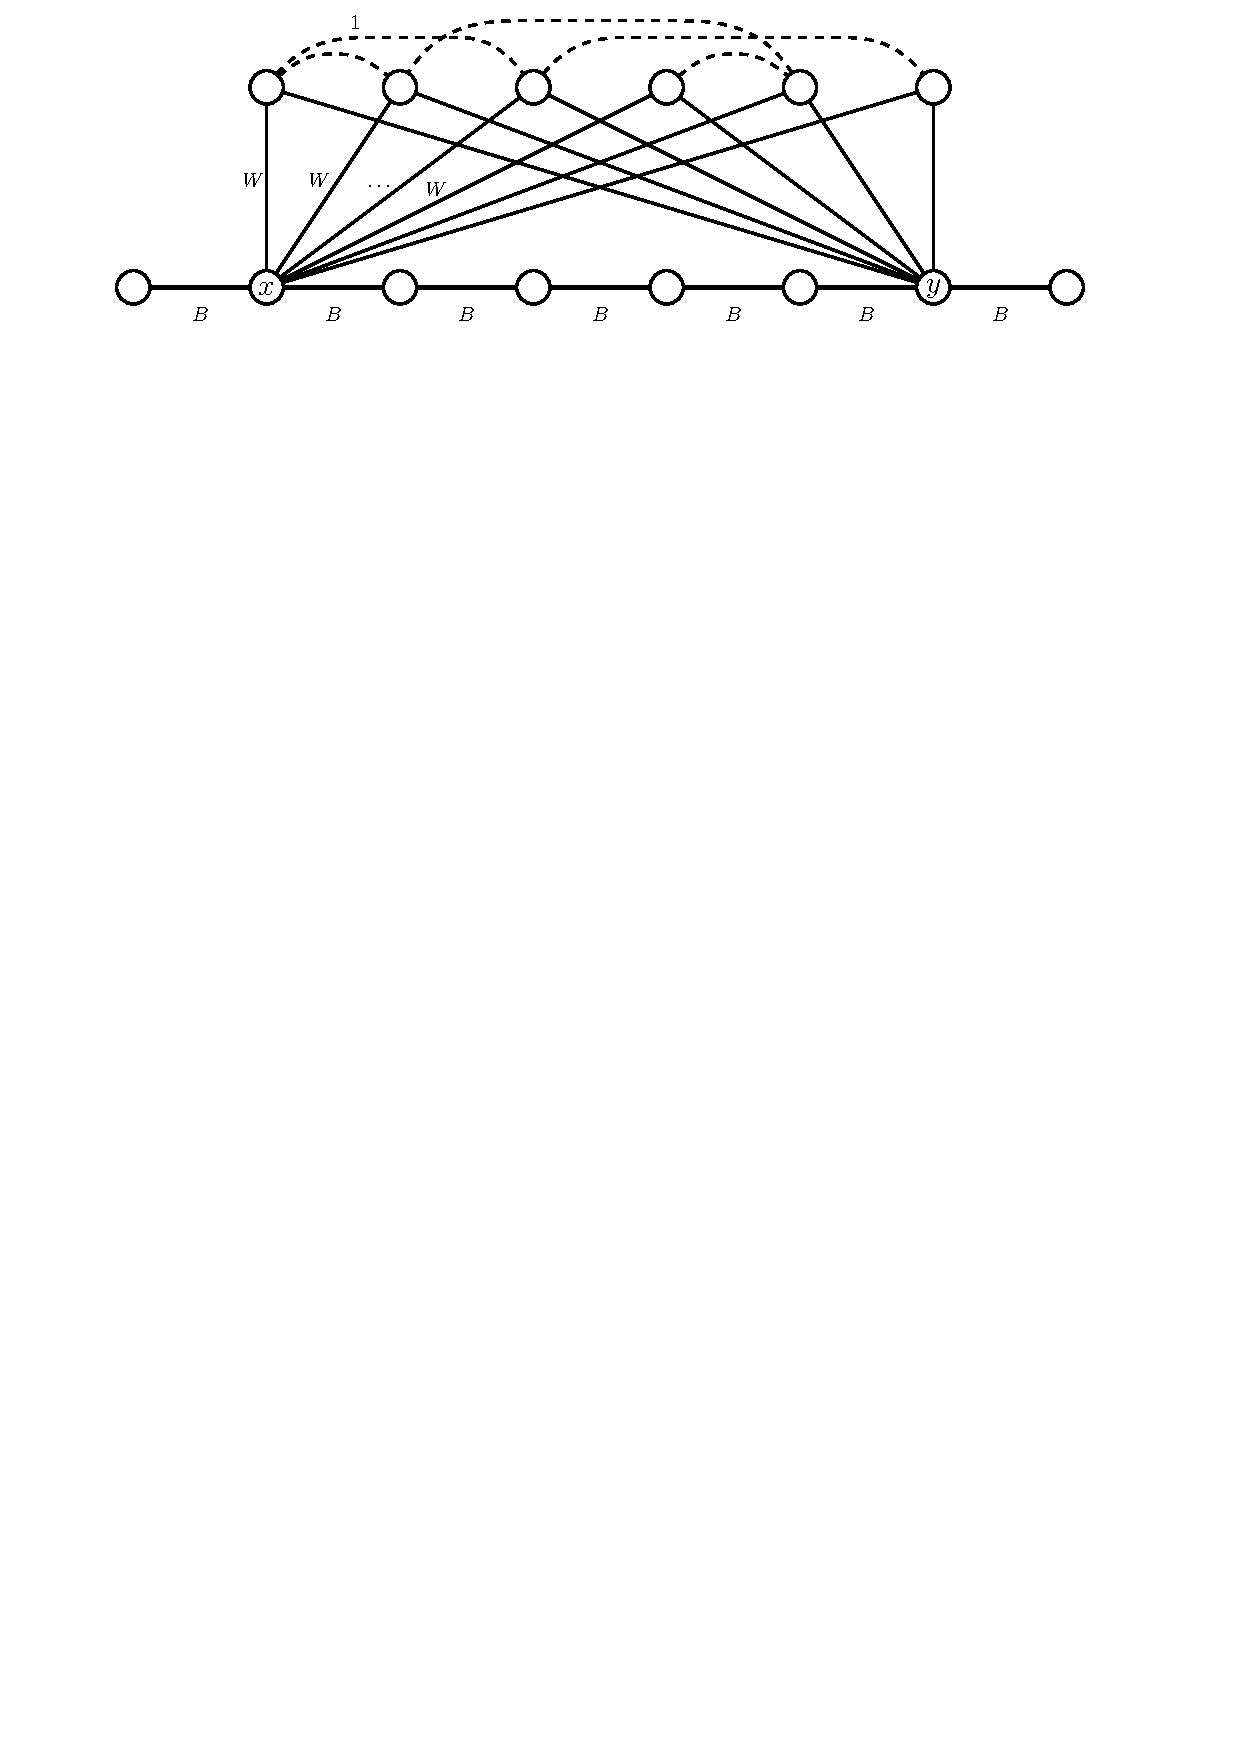
\includegraphics[width=0.3\textwidth]{figs/substitute}
%	\caption{Cluster types used in the analysis of \TAlg.}
%\end{figure}

\bibliographystyle{plainurl}
\bibliography{references}

\appendix


\end{document}
